\subsubsection{Registrovanje novog zaposlenog radnika}

\begin{itemize}
    \item Kratak opis:
        \begin{itemize}
            \item Administrator dodaje novog zaposlenog u sistem.
        \end{itemize}
    \item Učesnici:
        \begin{itemize}
            \item Administrator
        \end{itemize}
    \item Preduslovi:
        \begin{itemize}
            \item Sistem je u ispravnom stanju.
            \item Administrator poseduje informacije o novozaposlenom.
        \end{itemize}
    \item Postuslovi:
        \begin{itemize}
            \item Novi zaposleni je dodat u sistem i dobio je svoj lični nalog. Podaci su uspešno sačuvani u bazi podataka.
        \end{itemize}
    \item Osnovni tok:
        \begin{enumerate}
         \item Administrator otvara formu za unos podataka.
         \item Administrator vrši validaciju podataka.
         \item Administrator bira vrstu zaposlenog: koordinator, magacioner, dostavljač.
         \item Administrator unosi neophodne podatke i bira opciju ``Dodaj zaposlenog''.
         \item Sistem čuva unete podatke.
         \item Sistem šalje mejl zaposlenom sa linkom za početno pristupanje nalogu.
         \item Sistem obaveštava administratora o uspešnom dodavanju novog zaposlenog.
        \end{enumerate}
    \item Alternativni tok:
        \begin{itemize}
            \item[2.a] Administrator je uočio nepravilnost u prikupljenim podacima. Administrator kontaktira zaposlenog kako bi dobio ispravne podatke i ispravio ih u formi. Proces se nastavlja u 2. koraku osnovnog toka.
            \item[6.a] Zaposleni nije dobio mejl za pristupanje svom nalogu. Administrator zahteva od sistema da ponovo pošalje mejl. Proces se nastavlja u 6. koraku osnovnog toka.
        \end{itemize}
    \item Dodatne informacije:
        \begin{itemize}
            \item Podaci koji su neophodni za registraciju novog zaposlenog su: ime, prezime, mejl, telefon, jmbg.
        \end{itemize}
\end{itemize}

\begin{figure}[H]
\begin{center}
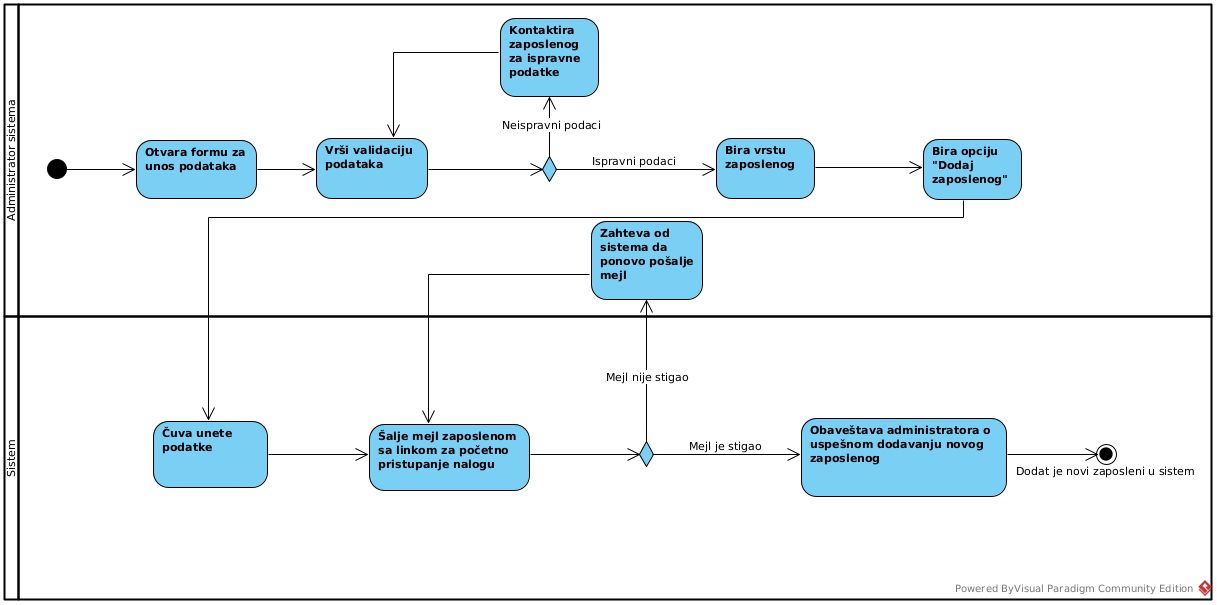
\includegraphics[width=\textwidth]{Pictures/activity_employee_registration.png}
\end{center}
    \caption{Dijagram aktivnosti registrovanje novog zaposlenog radnika}
\label{fig:ActivityEmployeeRegistration}
\end{figure}
